    \documentclass[conference]{IEEEtran}

    %%%%%%%%%%%%%%%%%%%%%%%%%%%%%%%%%%%%%%%%%%%%%%%%%%%%%%%%%%%%%%%%%%%%%%%%%%%%%
    %                              My Commands
    \newcommand{\bi}{\begin{itemize}}
    \newcommand{\ei}{\end{itemize}}
    \newcommand{\be}{\begin{enumerate}}
    \newcommand{\ee}{\end{enumerate}}
    \newcommand{\ii}{\item}
    \newtheorem{Def}{Definition}
    \newtheorem{Lem}{Lemma}

    \usepackage{algorithm}
    \usepackage{algorithmicx}
    \usepackage{algpseudocode}

    \usepackage{graphicx}
 
    \graphicspath{%
        {converted_graphics/}% inserted by PCTeX
        {./images/}% inserted by PCTeX
    }
    \usepackage{times}

    \begin{document}
    %
    % paper title
    % can use linebreaks \\ within to get better formatting as desired
    \title{Multi-view Rendering Approach for Cloud-based Gaming Services}

    % author names and affiliations
    % use a multiple column layout for up to three different
    % affiliations
    \author{\IEEEauthorblockN{Sung-Soo Kim, Kyoung-Ill Kim and Jongho Won}
    \IEEEauthorblockA{
            Electronics and Telecommunications Research Institute (ETRI)\\
            Daejeon, South Korea \\
            {\it \{sungsoo, kki, jhwon\}@etri.re.kr}
    }
    }

    % make the title area
    \maketitle

    \begin{abstract}
    In order to render hundreds or thousands of views for multi-user games on a cloud-based gaming at interactive rates, we need a solution which is both scalable and efficient.
    We present a new cloud-based gaming service system which supports
%    multi-view rendering for the multi-user games.
%    The goal of our research is to provide a new cloud-based gaming service that support
    multiple viewpoint rendering for visualizing a 3D game scene dataset at the same time for the multi-user games.
%    The proposed
    Our multi-view rendering algorithm maps well to the current graphics processing units (GPUs) and we have evaluated its performance on two different GPUs with different rendering resolution.
    The experimental results demonstrate the multi-view rendering method can be successfully applied to the multi-user games.
    \end{abstract}

    \begin{IEEEkeywords}
    gaming on demand, multi-view rendering, video encoding, video streaming, cloud computing
    \end{IEEEkeywords}

    \IEEEpeerreviewmaketitle
    \section{Introduction}
    \label{sc:Introduction}
    Cloud computing is a general term for complete services delivered over the networks using self-service end user portals and flexible business model that incorporates hardware, software, and services into a single revenue stream.
%    The growth in connectivity and capacity of broadband networks have enabled new forms of cloud computing where data and processing on a remote server is acted upon on a local computing device.
    This computing model allows a performance focus at a single location, the cloud server, and enables user mobility and pervasive access for the users.
    One of the latest advancements in gaming technology that enables such a ubiquitous gaming are \emph{cloud-based gaming service systems}, also called \emph{Gaming on Demand} (GoD) \cite{Jurgelionis:2009}.
    They are networked media platforms that offer web-based services allowing game play on smaller end-devices like low-cost PCs or set top boxes without requiring the games to be installed locally.

    The ultimate goal of the cloud-based gaming services is to provide pervasive game access on devices such as set top boxes and mobile devices that typically do not have a full set of technical requirements to run high-quality video games.
    This goal can be achieved by processing the game execution logic such as rendering, audio, artificial intelligence (AI) and physics, on at remote high-end servers
    being streamed as an interactive video over a network to be played on lightweight clients.
    Recent work in this area has been focused on video encoding and streaming techniques to reduce the latency in games.
%    such as \emph{3D graphics streaming} and \emph{video streaming} to reduce the latency in games.
    Most of the earlier systems were serial in nature and designed for a single core or processor in terms of 3D rendering.
     The recent trend in computer architecture has been toward developing parallel commodity processors, including multi-core CPUs and many-core GPUs.
    It is expected that the number of cores would increase at the rate corresponding to Moore's Law.
    Based on these trends, many parallel game engines \cite{Smoke:2009} and parallel rendering algorithms \cite{Humphreys:2002}\cite{Eilemann:2009} have been proposed for commodity parallel processors.

    In this paper, we propose a new cloud-based gaming service system to support the multi-view rendering based on multi-threaded game engine \cite{Smoke:2009} for the multi-user games.
    To provide convincing streaming-based GoD services, we describe the key requirements of cloud-based service systems as follows:
    \bi
    \ii \emph{User responsiveness}: Latency is defined as the time between a player's action and the time the actual resulting game output on the player's screen. Since computer games are highly interactive, extremely low latency has to be achieved.
%    In case of the first-person shooting (FPS) game, the threshold of latency is below 100 msec
    The interaction delay in the games should be kept below 80ms in order to guarantee suitable user responsiveness \cite{Claypool:2006}.
    \ii \emph{High-quality video}: In order to provide a high-quality video (above 720p) interactively, data shall be reduced as much as possible but keeping quality. However, video encoding is computationally quite demanding.
    \ii \emph{Quality of services}: In the case of network congestion, the network problems like increased latency, jitter, and packet losses distribute evenly on all competing traffic. However, the quality can be enhanced using quality of service (QoS) technologies to giver higher priority to game traffic in the network bottlenecks \cite{Jurgelionis:2010}.
    \ii \emph{Operating costs}: Since the servers of cloud-based gaming service system have high-performance CPUs and GPUs, the operating costs for the servers are quite expensive. So, it is necessary to develop the optimization technologies to minimize power consumption and network bandwidth \cite{Perlman:2009}.
%    Also, the dedicated hardware and software for video encoding and streaming can allow users to share common resources.
    \ei

    \noindent
    \textbf{Our contributions:} We present a novel system architecture for the cloud-based gaming services, which utilizes parallel commodity processors, multi-core CPUs.
    %as well as many-core GPUs.
    We also present a novel \emph{multi-view rendering} algorithm to efficiently support multi-user game on the server, which has a single GPU with multi-core CPUs.
    Our algorithm can easily handle insertion and removal of viewpoints and can also take advantage of scalable and parallel processing using multi-core CPUs.
    In addition, our approach give the benefits in terms of \emph{arbitrary focal positions} for viewpoints and better rendering quality over prior parallel multi-view rendering methods \cite{Lages:2008}.

    The rest of the paper is organized as follows.
    We briefly survey previous work on Gaming on Demand (GoD), parallel rendering and video encoding for the cloud-based gaming services in Section \ref{sc:RelatedWork}.
    Section \ref{sc:Architecture} describes the proposed the system architecture and the core systems in our system.
    We explain implementation details of our multi-view rendering algorithm and describe the performance result in Section \ref{sc:Implementation}.
    In Section \ref{sc:Comparison}, we compare our system and algorithm with prior GPU-based algorithms and highlight some of the benefits.
    Finally, we discuss future work and conclude in Section \ref{sc:Conclusion}.

    \section{Related work}
    \label{sc:RelatedWork}
    In this section, we give a brief overview of related work on cloud-based gaming technology and parallel rendering algorithms.
    We also highlight many technical characteristics of cloud-based gaming services, parallel rendering and video encoding.\\

    \noindent
    \textbf{Gaming on Demand (GoD):}
    There are a number of commercial Gaming on Demand systems that have been presented to the market \cite{Jurgelionis:2010}.
   % OnLive
   OnLive is a gaming-on-demand entertainment platform, announced at the Game Developers Conference (GDC) in 2009 \cite{Perlman:2009}.
%   Currently, their gaming service is available in USA.
%   They provide their service to clients nearby 1000-mile reach at five OnLive data centers in USA.
   % Gaikai
   Gaikai launched GoD beta service; \emph{Gaikai beta}, based on a cloud-based gaming technology that allows users to play major PC and console games \cite{Gaikai:2010}.
   The clients of their service can display audio/video (AV) game streams, which were streamed from the cloud, by using previously installed plug-ins such as Java or Adobe Flash on client devices.
   Even though both are cloud base gaming, OnLive and Gaikai have different goals in mind.
   OnLive sells full games, provides demos, brag clips, and being able to watch other players play games (Arena) while Gaikai advertises games via a webpage as demos \cite{Perlman:2009}.

   % OTOY
%   OTOY provides technologies that move processor intensive experiences into the cloud; computer applications, operating system, video games, high-definition (HD) media content, film/video special effects graphics - fully interactive, in real time, through the power of \emph{server side rendering} \cite{OTOY:2009}.
   Visual effects rendering based on \emph{global illumination} that commonly requires extensive hardware and processing time.
%   However, their system can provide visual effects rendering in real-time using their cloud; \emph{Fusion Render Cloud} (FRC).
   However, the OTOY can provide visual effects rendering in real-time using the cloud; \emph{Fusion Render Cloud} (FRC), through the power of \emph{server side rendering} \cite{OTOY:2009}.
%   They can deliver the high-quality media content via an interactive stream to any internet enabled device, including PC, iPhone, iPad or TV set top box.
   However, there is very little detailed technical information publicly available about these commercial systems.

   % Game@Large
   The \emph{Games@Large} (G@L) framework enables commercial video game streaming from a local server to remote end devices in local area networks (LANs) \cite{Tzruya:2006}.
   This system and streaming protocols are developed and adapted for highly interactive video games \cite{Jurgelionis:2009} \cite{Nave:2008}.

   There are two major approaches for the game streaming.
   One is \emph{3D graphics streaming} approach which exploited for streaming the game's output is to directly transmit the graphics commands to the client device and render the image on the client device \cite{Humphreys:2002}.
   The other approach is \emph{video streaming} that the server renders the game graphics scene, the framebuffer is captured, eventually downsampled to match the target resolution, and the current image is encoded using standard video codes such as MPEG-2, MPEG-4 and H.264 \cite{Cheng:2004}\cite{Karachristos:2008}.
   The video streaming is intended for thin-client devices lacking hardware accelerated rendering capabilities \cite{Winter:2006}.
%   The G@L framework supported these two streaming methods \cite{Jurgelionis:2009}\cite{Nave:2008}.
   In our research, we exploit a video streaming method since our system should support the thin-client devices.\\

    \noindent
    \textbf{Parallel rendering:}
%    Parallel computing is quickly becoming mainstream. Dual-core and quad-core CPU chips are currently available, with some motherboards supporting multiple such chips.
    Much of the recent work in the area of parallel rendering has focused on using networked clusters of commodity PCs.
    Such systems can generally drive a tiled display using a commodity local network as well.
%    High-quality 3D games are important in entertainment applications of computer graphics in commercial game industry.
    There are three major approaches according to a sorting classification of parallel rendering such as \emph{sort-first}, \emph{sort-middle} and \emph{sort-last rendering} \cite{Molnar:2008}.

    Also, there have been various research efforts to multi-view rendering and scalable rendering \cite{Eilemann:2009}.
    However, those methods cannot be directly employed for multi-view rendering for multi-user games
    since those methods usually focus on multipipe display systems, workstations with multiple monitors, walls build out of multiple screens or projectors as well as immersive environments.

    A parallel multi-view rendering architecture in a cluster of GPUs has been proposed in \cite{Lages:2008}.
    This system have shown a theoretical analysis of speedup and scalability of the proposed multi-view rendering.
    However, the critical limitation of this method is that all the cameras are always looking to the center of arbitrary tile.
    This is not suitable for common mutli-user game applications.
    Moreover, it is difficult to apply this method to a \emph{high visual quality} (photo-realistic) games  since they used a simple phong shader for lighting and shading.

    In this paper, we exploit a parallel game engine for improving the multi-view rendering performance as well as the visual realism in the games as shown in Fig. \ref{fig:multi-view}.\\

    \begin{figure*}[tbh] % float placement: (h)ere, page (t)op, page (b)ottom, other (p)age
    \centering
    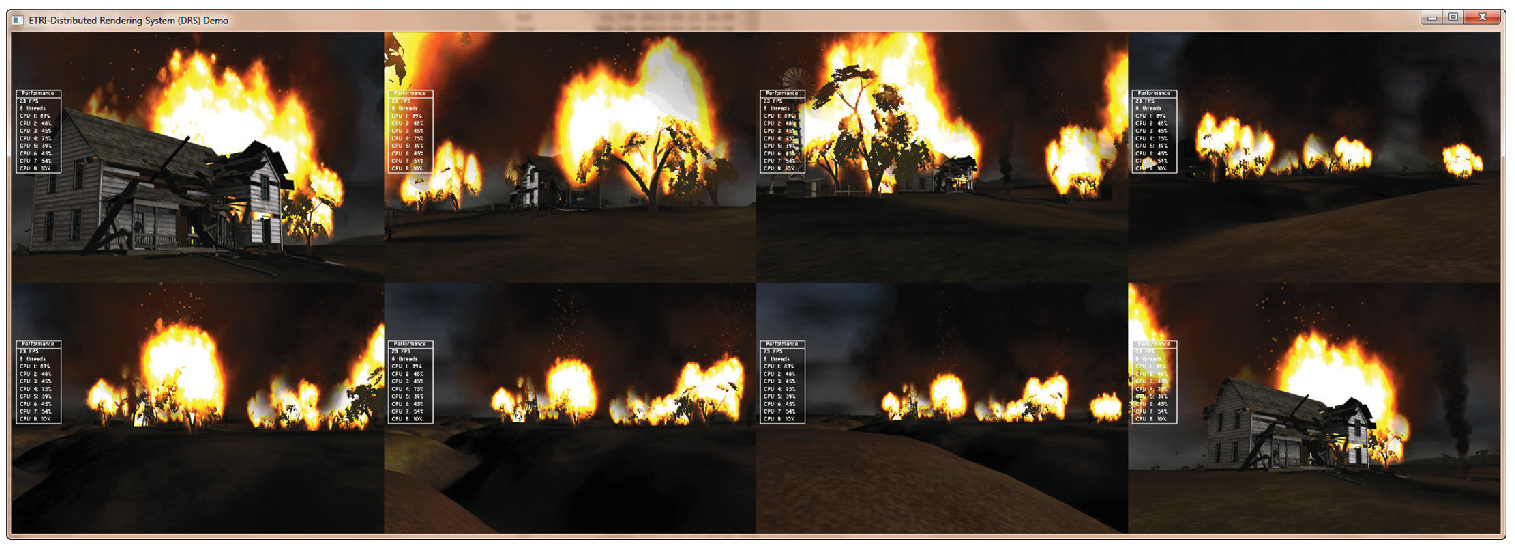
\includegraphics[height=5.8cm,keepaspectratio]{eight-view}
    \caption{The result of our multi-view rendering algorithm (eight views with 640x480 resolution for each view.)}
    \label{fig:multi-view}
    \end{figure*}

    \noindent
    \textbf{Video encoding:}
    % Research papers
    Many techniques have been proposed to accelerate the performance of video encoding algorithms.
%    In order to minimize the efforts needed to integrate new client devices the streamed game video data is fully compliant to standard codec such as MPEG-4 and H.264.
    In H.264/AVC encoders, \emph{macroblock partitioning} and \emph{motion vector calculation} are computationally very demanding.
    An acceleration based on render context information has been developed, which allows the direct calculation of motion vectors, similar to \cite{Cheng:2004}.
%    Zrida et. al proposed the parallel model of the encoder using multiprocessor platforms \cite{Zrida:2009}.
    The parallel model of the encoder using multiprocessor platforms has been introduced in order to improve the encoding performance in \cite{Zrida:2009}.

    % OnLive
    OnLive introduced \emph{interactive video compression} method designed for video games.
%    This method works reliably on home broadband connections in USA.
    In order to achieve high performance encoding, they developed two dedicated compression hardware for video encoding;
    \emph{optimized compressor} based on \emph{human perception} and \emph{live compressor} similar to conventional compressor \cite{Perlman:2009}.

    % OTOY
%    Unlike H.264, which was designed in 2003 to take advantage of specialized hardware for encoding and decoding video.
    Current GPUs are regards as high-throughput processors, which have a theoretical peak performance of a few Tera-Flops. In order to accelerate the performance of the motion estimation, fast motion estimation implementation using CUDA on GPU has been proposed in \cite{Colic:2010}.
    Recently, OTOY introduced new video encoding method, so-called \emph{ORBX}.
    ORBX has been designed from the ground up to take advantage of OpenCL based GPU servers (FRC). ORBX encodes video entirely on the GPU, with more than 30-100x the scaling of H.264 encoding solutions requiring either a CPU or specialized encoding ASIC \cite{OTOY:2009}.
    Unfortunately, the technical information of the ORBX encoding method is not publicly available.

    \section{System Architecture}
    \label{sc:Architecture}
    In this section, we describe the proposed system architecture for the cloud-based gaming services.
    Our architecture consists of three major systems such as distributed service platform (DSP), distributed rendering system (DRS) and encoding/QoS/streaming system (EQS) as shown in Fig. \ref{fig:architecture}.

    \subsection{System Overview}
    \label{sub:Overview}
    % overview
    % DSP role
    The Distributed Service Platform (DSP) is responsible for launching the game processes on the game execution nodes or rendering job on the Distributed Rendering System (DRS) after client-side invocation, monitoring its performance, allocating computing resources and managing user information.
    And, the DSP is responsible for processing user's game input via UDP from the client-side devices.
    In client-side, the user's game input is captured and transmitted via UDP by the user input capturing and transmission software on the client devices.
    Also, the DSP performs execution management of multiple games.
    In order to perform streaming the game A/V streams to the clients, the DSP requests capturing rendered frame buffer for video encoding and streaming to the Encoding/QoS/Streaming System (EQS).
    \begin{figure}[htb] % float placement: (h)ere, page (t)op, page (b)ottom, other (p)age
    \centering
    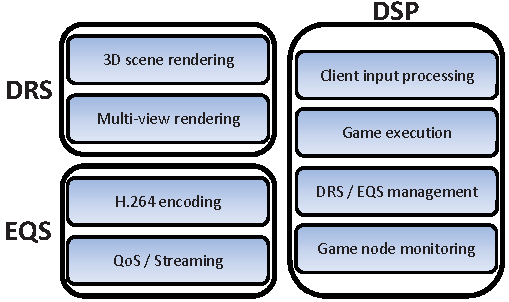
\includegraphics[width=7cm,height=5.24cm,keepaspectratio]{figure01}
    \caption{Our system architecture: \emph{DSP-Distributed Service Platform, DRS-Distributed Rendering System, EQS-Encoding, QoS and Streaming System}}
    \label{fig:architecture}
    \end{figure}

    % DRS role
    The DRS is responsible for rendering a 3D scene and \emph{multi-view rendering} for multi-user games.
    To improve 3D rendering performance in games, we utilize the multi-threaded game engine \cite{Smoke:2009} that is designed to scale to as many processors as are available within a platform.

    % EQS role
    The EQS is responsible for audio/video encoding and streaming the interactive game content to the clients.
    In order to implement the visual capturing for the games, we utilize the DirectShow SDK.
    And we utilize the H.264 video coding standard for low-delay video encoding of the captured game content.
    Before the EQS performs the H.264 encoding, we perform a color space conversion from RGB to YUV on the captured frames.
    Finally, we exploit the Real Time Protocol (RTP) packetization to transmit the encoded video stream in real-time \cite{RTP50}\cite{RTP84}.
    \begin{figure}[htb] % float placement: (h)ere, page (t)op, page (b)ottom, other (p)age
    \centering
    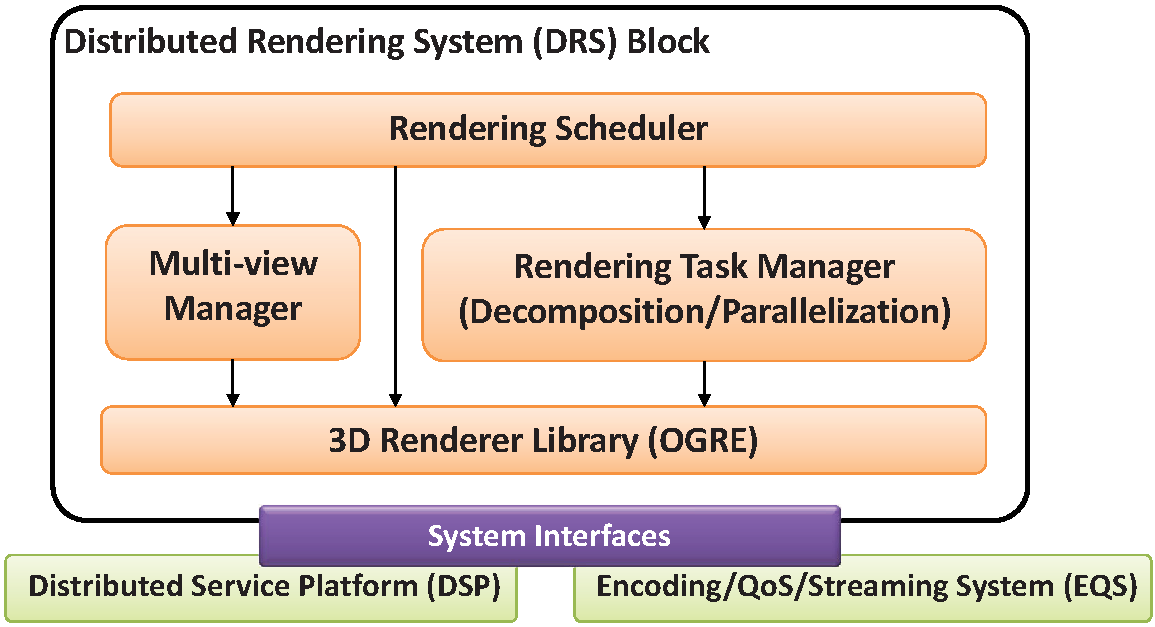
\includegraphics[width=8cm, keepaspectratio]{DRSblock}
    \caption{The DRS block architecture}
    \label{fig:DRS}
    \end{figure}

    \subsection{Distributed Rendering System}
    \label{sub:DRS}
    The Distributed Rendering System (DRS) consists of four major block components such as \emph{rendering scheduler}, \emph{multi-view manager}, \emph{rendering task manager} and \emph{renderer library} as shown in Fig. \ref{fig:DRS}. The rendering scheduler is responsible for rendering process monitoring, performance timer control, rendering statistics management and communicating other modules for external rendering requests in the DRS blocks. The key performance improvements for the game applications is the use of per-thread task queues. This eliminates the synchronization checkpoint when one shared task queue is used.
    Advanced task schedulers may use heuristics to determine which thread to steal from and which task to steal and this may help cache performance.
    In order to implement the rendering scheduler, we use the Intel Threading Building Blocks (TBB) \cite{TBB:2010}, which is highly optimized scheduler for Windows, Mac OS X, and Linux.
    The multi-view manager is responsible for performing the management of user's viewpoints (such as insertion, deletion, update and search operations) for the shared spaces in the multi-user games.
    The rendering task manager module performs the rendering task decomposition and parallelization in order to improve the rendering performance.
    In our work, we use the Object-oriented Graphics Rendering Engine (OGRE) \cite{OGRE:2010}, which performs a 3D scene graph management and rendering.
    In order to provide the cloud-based gaming service, the DRS should have common system interfaces to the DSP and the EQS.

    \subsection{Multi-view Rendering}
    \label{sub:multiview}
    In the case of multi-user games, multiple viewpoints are needed if we want to support several users visualizing a given 3D scene at the same time.
    However, rendering multiple views using the standard graphics pipeline is a challenging problem.

    In order to provide the interactive multi-view rendering results for the cloud-based gaming service,
    we utilized the shared resources for the rendering such as scene graph, textures and shaders in a GPU as much as possible and keeping the quality of the rendering results.

    If $R_i$ denotes a $i$-th rendered image in framebuffer of the DRS, then $\mathcal{S}_k$, which has $i$ image sequences is defined as:
    $$ \mathcal{S}_k = \{R_1, R_2, ... , R_i \} $$
    The $\mathcal{CP}_i$ denotes the $i$-th viewpoint parameters, which contains internal parameters
    such as focal length $f_l(f_x, f_y)$, center $c(c_x, c_y)$, aspect ratio $a$ and external parameters
    such as position $p(c_x, c_y, c_z)$ and orientation $r(r_x, r_y, r_z)$. The DSP generates this $\mathcal{CP}_i$ according to the requests of the clients.
    \begin{algorithm}
    \caption{Viewpoint addition algorithm.}
    \label{algo:addview}
    \begin{algorithmic}[1]
    \Procedure{AddView}{$U_{i}, \mathcal{CP}_i$}
       \State RenderWindow $W$;
       \State Camera $C_i$;
       \State Viewport $V_i$;
       \State RenderedFrameBuffer $R_i$;
       \State $C_i \gets$ createCamera($U_i$, $\mathcal{CP}_i$);
       \State $V_i \gets$ addViewport($C_i$);
       \State $R_i \gets$ renderOneFrame($W, V_i, C_i$);
       \State \textbf{return} $R_i$
    \EndProcedure
    \end{algorithmic}
    \end{algorithm}

    The DRS provides the function for adding the multiple viewpoints to support the multi-view rendering.
    First, the DSP receive the service requests from the clients. These requests include several user information, $U_i$, such as user identification, selected game, which they want to play and initial or previous viewpoints in the 3D game space. Then, the DSP sends these information to the DRS to request for multi-view rendering. According to this request, the DRS provides the function for adding viewpoints, $\mathcal{CP}_i$. To perform this function on the DRS, we create the cameara $C_i$ and viewport $V_i$ objects to attach the viewport to the render window $W_i$. After the viewport was successfully added to the render window, the DRS performs the rendering procedure to generate an image on the framebuffer in a GPU. The pipeline of our algorithm for multi-view rendering is shown in \textbf{Algorithm \ref{algo:addview}}.
    Another function for multi-view rendering is deletion function for viewpoints in the multi-user games. This function can be easily implemented similar to the viewpoint addition algorithm.

    If $EA_i$ and $EV_i$ denote a $i$-th encoded audio and video in interactive game content respectively,
    then $\mathcal{ES}_k$, which has $i$ encoded audio/visual gaming sequences is defined as:
    $$ \mathcal{ES}_k = \{(EA_1, EV_1), (EA_2, EV_2), ... , (EA_i, EV_i) \} $$
    Therefore, the EQS performs the streaming $ \mathcal{ES}_k$ to the clients for the cloud-based gaming services.
    In order to  address the game's audio/visual output capturing, we develop the capturing module on the EQS in C++ and DirectShow SDK.
    We also develop the H.264 encoder for achieving low-delay video coding.
    \begin{algorithm}
    \caption{Video encoding and streaming algorithm.}
    \label{algo:encoding}
    \begin{algorithmic}[1]
    \Procedure{EncodingAndStreaming}{$U_{i}$}
       \State YUVImage $Y_i$;
       \State FrameCapture $F_i$;
       \State FrameNumber $f$;
       \State EncodedAudio $EA_i$;
       \State EncodedVideo $EV_i$;
       \State $F_i \gets$ captureRenderedFrameBuffer($U_i$, $f$); \label{state:capture}
       \While{$F_i \not=$ NULL}
            \State $Y_i \gets$ convertRGB2YUV($F_i$);
            \State $EV_i \gets$ encodeFrame($Y_i$);
            \State $EA_i \gets$ captureAndencodeAudio($U_i$, $f$);
            \State $\mathcal{ES}_i \gets$ transmitAVstream($EA_i$, $EV_i$, $f$);
            \State $F_i \gets$ captureRenderedFrameBuffer($U_i$,$f$);
       \EndWhile
    \EndProcedure
    \end{algorithmic}
    \end{algorithm}
    Before the EQS performs the H.264 encoding, a color space conversion from RGB to YUV (convertRGB2YUV function in \textbf{Algorithm \ref{algo:encoding}}) takes place on the captured frames $F_i$. We utilized the 4:2:0 method for the YUV sampling to achieve the reduction of storage data.
    We also capture and encode the audio data for the games to transmit the interactive game content to the clients. In our work, HE-AACv2 is utilized for audio streaming. And then, the EQS transmits the encoded AV content for the game to the client via RTP/RTCP \cite{RTP84}. The details of our video encoding and streaming algorithm for interactive gaming content is shown in \textbf{Algorithm \ref{algo:encoding}}.

    On the other hand, the client side devices for our system support the H.264 decoding functionality.
    Also, the client is responsible for capturing the commands of the input controller such as keyboard and mouse, and sending them to the DSP via UDP.
    \section{Implementation and Performance}
    \label{sc:Implementation}
    In this section, we describe the implementation of our system and highlight the performance of our multi-view algorithm.\\

    \noindent
    \textbf{Implementation:} We have implemented our multi-view algorithm on two different commodity GPUs: a NVIDIA GTX 480, a NVIDIA Quadro 4000.
    \begin{figure}[htb] % float placement: (h)ere, page (t)op, page (b)ottom, other (p)age
    \centering
    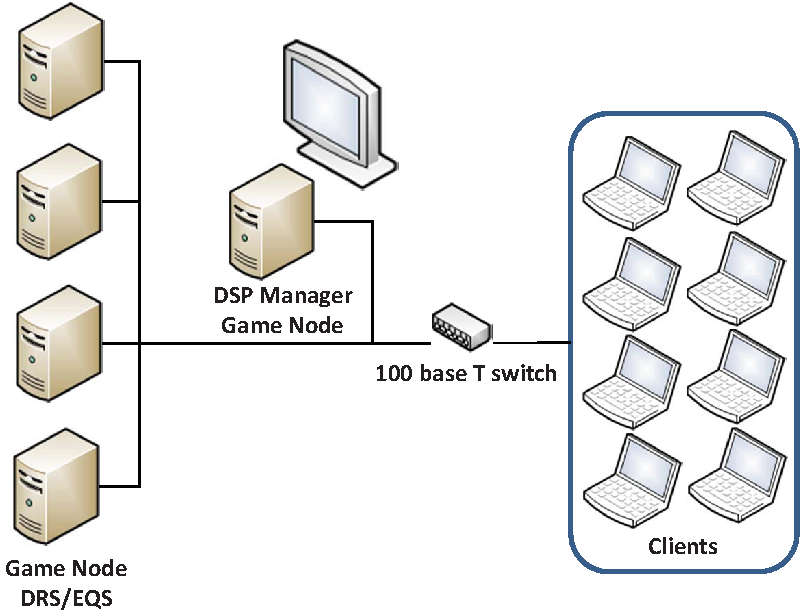
\includegraphics[width=7cm, keepaspectratio]{testenv}
    \caption{Performance test setup: \emph{This figure shows the system configuration; five workstations for servers, eight laptops as thin-clients, for the performance testing.}}
    \label{fig:testenv}
    \end{figure}
    In order to test the performance of our system, we used five workstations (Intel Core i7, 8G RAM) which were connected to a 100 Mbps switch via a wired Ethernet connection. Also, the eight laptops as thin-clients (Intel 2GHz, 1G RAM) were connected to the 100Mbit LAN. These laptops are capable of H.264 decoding and displaying the game videostream as shown in Fig. \ref{fig:testenv}.

    \begin{figure}[htb] % float placement: (h)ere, page (t)op, page (b)ottom, other (p)age
    \centering
    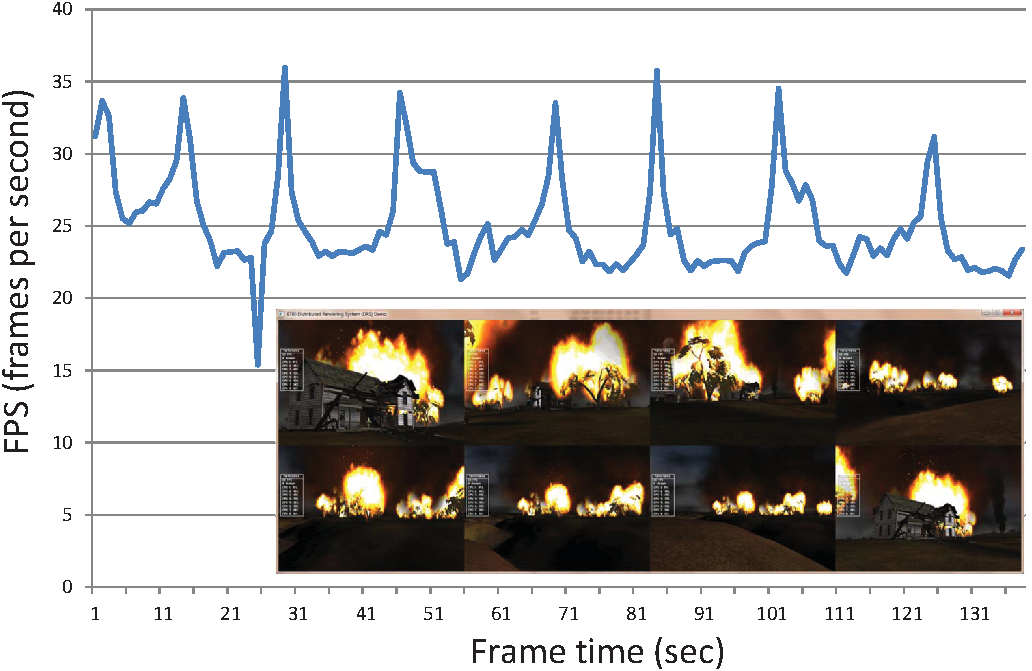
\includegraphics[width=7.5cm, keepaspectratio]{performancegraph}
    \caption{Performance of multi-view rendering: \emph{This figure shows the frames per second (fps); 25.4 on average, for multi-view rendering (640x480 resolution for each view) on a NVIDIA Quadro 4000.}}
    \label{fig:graph}
    \end{figure}

    \noindent
    \textbf{Performance:}
    First we evaluate the performance of multi-view rendering on a PC running Windows 7 operating system with Intel Core i7 2.93GHz CPU, 8GB memory and a NVIDIA Quadro 4000. We used OGRE library based on DirectX as a graphics API and Microsoft HLSL for a shading language.

    The frames for second (FPS) is the number of frames per second that have been rendered by the DRS.
    High FPS results with smooth movements in the 3D scene.
    Our system rendered 8 views at 25.4 fps on average with one GPU.
    We measured the FPS every second at the DRS for rendering at 640x480 resolution for each view.
    Fig. \ref{fig:graph} shows the performance result of multi-view rendering.

    We utilized the parallel game engine; \emph{Intel Smoke} \cite{Smoke:2009}, and we adopted our multi-view rendering algorithm.
    Then we ran it on a 8 core system with a NVIDIA GTX 480 to measure the scalability of our rendering system as shown in Fig. \ref{fig:scaling}.
    \begin{figure}[htb] % float placement: (h)ere, page (t)op, page (b)ottom, other (p)age
    \centering
    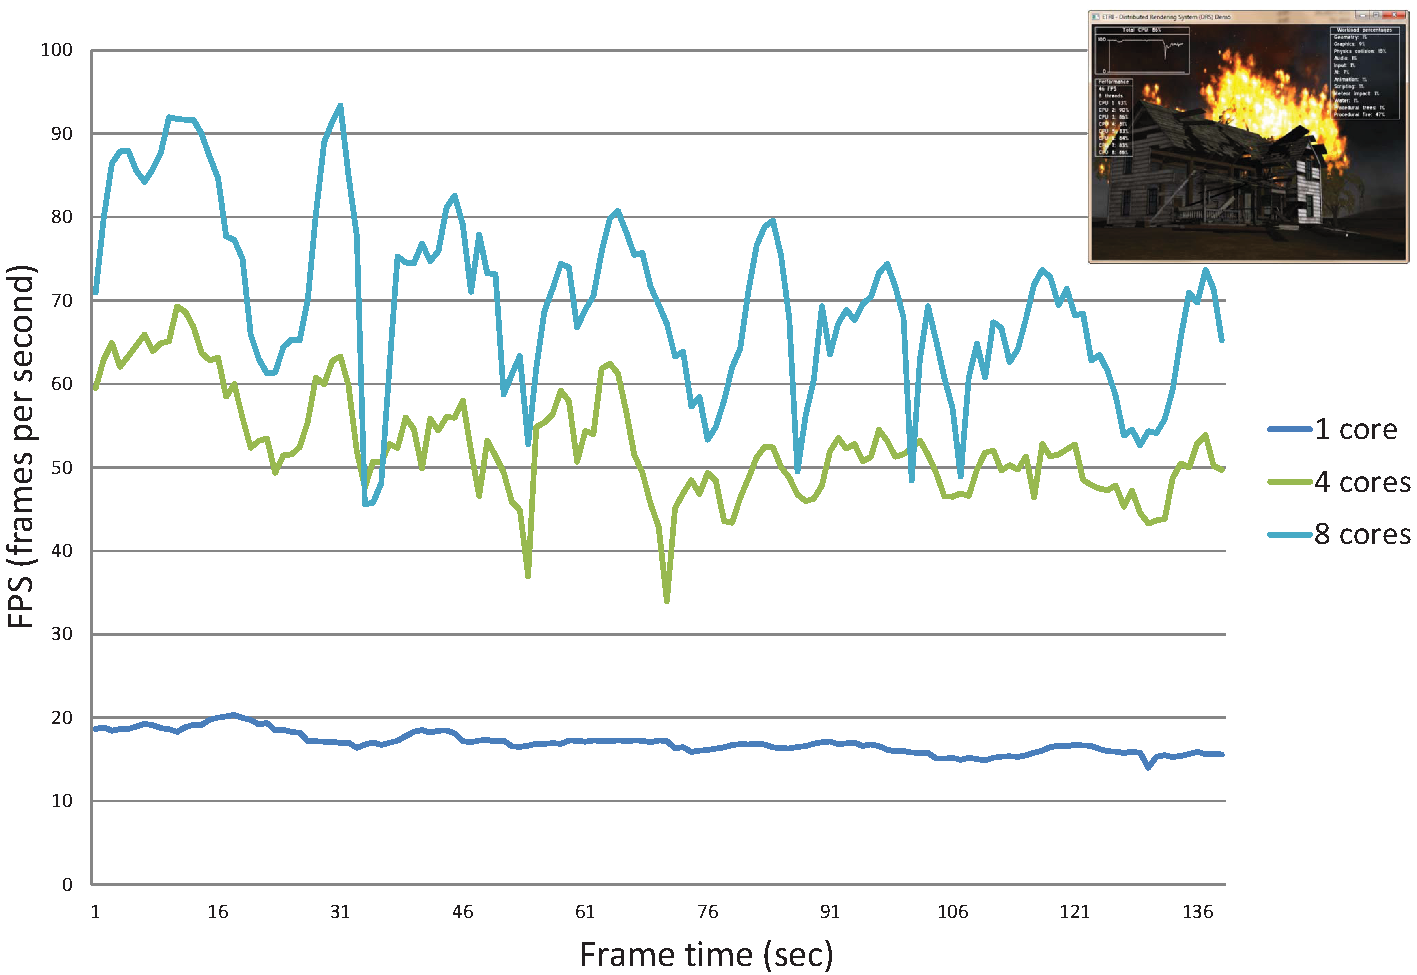
\includegraphics[width=7.51cm,keepaspectratio]{scalinggraph}
    \caption{Scaling performance of the DRS according to the number of CPU cores: \emph{This figure shows the scalability of our parallel (multi-threaded) rendering (1600x1200 resolution) on a Intel i7 8-core
    (quad-core with hyperthreading)
    with a NVIDIA GTX 480. Average FPS - 1 core: 16.9, 4 cores: 52.6, 8 cores: 69.7 }}
    \label{fig:scaling}
    \end{figure}

    In terms of the performance of our encoding system, our system can encode in 25.6ms on average for eight views (interactive gaming videos) with 640x480 resolution in parallel and 24.9ms for a 1600x1200 video.
    \textbf{Table \ref{tlb:EQSfeature}} shows the supported technical features of AV encoding in the proposed system.
    \begin{table}[htb]
    \caption{The supported features of audio/video encoding in our system.}
    \center{
    \begin{tabular}{l|c|c}\hline
    \textbf{Supported features}  & \textbf{Audio} & \textbf{Video} \\\hline\hline
    Codec & HE-AACv2 & MPEG-4, H.264 \\
    Resolution & - & 320x240 - 1600x1200 \\
    Bitrate & 16Kbps - 64Kbps & 384Kbps - 5Mbps \\
    Frame Rate & - & 5 - 30fps \\
    Sampling Rate & 22.05KHz - 48KHz & - \\
    Channel & Mono, Stereo & - \\\hline
    \end{tabular}
    }
    \label{tlb:EQSfeature}
    \end{table}

%    \section{Comparison and Analysis}
    \section{Analysis}
    \label{sc:Comparison}
    In this section, we evaluate the performance of our system in terms of rendering and encoding functionalities and highlight some of the benefits.
    \\
%    \noindent
%    {\bf Comparison:}

    \noindent
    {\bf Analysis:} Our rendering system provides good performance scaling of multi-core CPUs for multi-view rendering.
    And the multi-view rendering algorithm maps well to the current GPUs and we have evaluated its performance on two different GPUs with different rendering resolution.
    Furthermore, it is relatively simple to combine the video encoding methods and optimizations in the streaming-based gaming service framework. This makes it possible to develop a more flexible GPU-based framework for the video encoding methods like H.264/AVC or ORBX which is GPU-based encoding schemes.\\

    \noindent
    {\bf Limitations:}
    Our approach has some limitations.
    First, we support the multi-view rendering for one multi-user game, since it is difficult to share the rendering resources in a GPU among different games. We believe that this can be resolved by using multi-GPUs.
    Secondly, our system performs directly rendering to the framebuffers on the server-side machines.
    However, in terms of efficient services in the cloud-based gaming, we should exploit the \emph{off-screen rendering} approaches and \emph{GPU virtualization} techniques.

    \section{Conclusion and Future Work}
    \label{sc:Conclusion}
    In this paper, we have presented a system architecture for the cloud-based gaming service and multi-view rendering.
%    Also, we have described a new technique for parallelized and distributed multi-view rendering.
    Our rendering system greatly improves utilization of hardware resources present in the system, allowing to utilize both multi-core CPUs and a GPU simultaneously.

    We found that the proposed system provide the multi-view rendering for different focal positions for each viewpoint with high visual quality.
    Moreover, our approach is flexible and maps well to current GPUs in terms of shared resources such as textures and shaders for rendering.
    In addition, we demonstrate that the proposed rendering system could prove to be scalable in terms of parallel rendering. So, we believe that our rendering system will provide high-quality with good performance for the cloud-based gaming services.

    There are many avenues for future work. It is possible to use new capabilities and optimizations to improve the performance of the video encoding especially H.264/AVC through the GPU-based implementation.
    Furthermore, we would like to develop algorithms for integrating the multi-view rendering with the video encoding in a GPU.
%    without a CPU-GPU I/O for the video encoding.

    % use section* for acknowledgement
    \section*{Acknowledgments}
    \label{sc:Acknowledgment}
    The game technology demo (Intel's smoke demo) in Fig. \ref{fig:multi-view} is courtesy of the Intel Corporation.
    The authors appreciate valuable comments for the development of the multi-view rendering algorithm from Dr. Choong-Gyu Lim.
    This work was supported in part by the SW computing R\&D program of MKE/KEIT [10035184], \emph{Game Service Technology Based on Realtime Streaming}.

    \bibliographystyle{IEEEtran}
    \bibliography{IEEEabrv,AFIN2011}


    % that's all folks
    \end{document}
